\documentclass[]{article}
\usepackage{lmodern}
\usepackage{amssymb,amsmath}
\usepackage{ifxetex,ifluatex}
\usepackage{fixltx2e} % provides \textsubscript
\ifnum 0\ifxetex 1\fi\ifluatex 1\fi=0 % if pdftex
  \usepackage[T1]{fontenc}
  \usepackage[utf8]{inputenc}
\else % if luatex or xelatex
  \ifxetex
    \usepackage{mathspec}
    \usepackage{xltxtra,xunicode}
  \else
    \usepackage{fontspec}
  \fi
  \defaultfontfeatures{Mapping=tex-text,Scale=MatchLowercase}
  \newcommand{\euro}{€}
\fi
% use upquote if available, for straight quotes in verbatim environments
\IfFileExists{upquote.sty}{\usepackage{upquote}}{}
% use microtype if available
\IfFileExists{microtype.sty}{%
\usepackage{microtype}
\UseMicrotypeSet[protrusion]{basicmath} % disable protrusion for tt fonts
}{}
\usepackage[margin=1in]{geometry}
\usepackage{natbib}
\bibliographystyle{plainnat}
\usepackage{color}
\usepackage{fancyvrb}
\newcommand{\VerbBar}{|}
\newcommand{\VERB}{\Verb[commandchars=\\\{\}]}
\DefineVerbatimEnvironment{Highlighting}{Verbatim}{commandchars=\\\{\}}
% Add ',fontsize=\small' for more characters per line
\usepackage{framed}
\definecolor{shadecolor}{RGB}{248,248,248}
\newenvironment{Shaded}{\begin{snugshade}}{\end{snugshade}}
\newcommand{\KeywordTok}[1]{\textcolor[rgb]{0.13,0.29,0.53}{\textbf{{#1}}}}
\newcommand{\DataTypeTok}[1]{\textcolor[rgb]{0.13,0.29,0.53}{{#1}}}
\newcommand{\DecValTok}[1]{\textcolor[rgb]{0.00,0.00,0.81}{{#1}}}
\newcommand{\BaseNTok}[1]{\textcolor[rgb]{0.00,0.00,0.81}{{#1}}}
\newcommand{\FloatTok}[1]{\textcolor[rgb]{0.00,0.00,0.81}{{#1}}}
\newcommand{\CharTok}[1]{\textcolor[rgb]{0.31,0.60,0.02}{{#1}}}
\newcommand{\StringTok}[1]{\textcolor[rgb]{0.31,0.60,0.02}{{#1}}}
\newcommand{\CommentTok}[1]{\textcolor[rgb]{0.56,0.35,0.01}{\textit{{#1}}}}
\newcommand{\OtherTok}[1]{\textcolor[rgb]{0.56,0.35,0.01}{{#1}}}
\newcommand{\AlertTok}[1]{\textcolor[rgb]{0.94,0.16,0.16}{{#1}}}
\newcommand{\FunctionTok}[1]{\textcolor[rgb]{0.00,0.00,0.00}{{#1}}}
\newcommand{\RegionMarkerTok}[1]{{#1}}
\newcommand{\ErrorTok}[1]{\textbf{{#1}}}
\newcommand{\NormalTok}[1]{{#1}}
\usepackage{longtable,booktabs}
\usepackage{graphicx}
\makeatletter
\def\maxwidth{\ifdim\Gin@nat@width>\linewidth\linewidth\else\Gin@nat@width\fi}
\def\maxheight{\ifdim\Gin@nat@height>\textheight\textheight\else\Gin@nat@height\fi}
\makeatother
% Scale images if necessary, so that they will not overflow the page
% margins by default, and it is still possible to overwrite the defaults
% using explicit options in \includegraphics[width, height, ...]{}
\setkeys{Gin}{width=\maxwidth,height=\maxheight,keepaspectratio}
\ifxetex
  \usepackage[setpagesize=false, % page size defined by xetex
              unicode=false, % unicode breaks when used with xetex
              xetex]{hyperref}
\else
  \usepackage[unicode=true]{hyperref}
\fi
\hypersetup{breaklinks=true,
            bookmarks=true,
            pdfauthor={by Kasper Welbers and Wouter van Atteveldt},
            pdftitle={Newsflow: An R package for analyzing content homogeneity and news diffusion using computational text analysis},
            colorlinks=true,
            citecolor=blue,
            urlcolor=blue,
            linkcolor=magenta,
            pdfborder={0 0 0}}
\urlstyle{same}  % don't use monospace font for urls
\setlength{\parindent}{0pt}
\setlength{\parskip}{6pt plus 2pt minus 1pt}
\setlength{\emergencystretch}{3em}  % prevent overfull lines
\setcounter{secnumdepth}{0}

%%% Use protect on footnotes to avoid problems with footnotes in titles
\let\rmarkdownfootnote\footnote%
\def\footnote{\protect\rmarkdownfootnote}

%%% Change title format to be more compact
\usepackage{titling}

% Create subtitle command for use in maketitle
\newcommand{\subtitle}[1]{
  \posttitle{
    \begin{center}\large#1\end{center}
    }
}

\setlength{\droptitle}{-2em}
  \title{Newsflow: An R package for analyzing content homogeneity and news
diffusion using computational text analysis}
  \pretitle{\vspace{\droptitle}\centering\huge}
  \posttitle{\par}
  \author{by Kasper Welbers and Wouter van Atteveldt}
  \preauthor{\centering\large\emph}
  \postauthor{\par}
  \date{}
  \predate{}\postdate{}



\begin{document}

\maketitle

\begin{abstract}
Given the sheer amount of news sources in the digital age (e.g.,
newspapers, blogs, social media) it has become difficult to determine
where news is first introduced and how it diffuses across sources. We
introduce Newsflow: an R package for analyzing content homogeneity and
diffusion patterns using computational text analysis. The content of
news messages is compared using techniques from the field of information
retrieval, similar to plagiarism detection. By using a sliding window
approach to only compare messages within a given time distance, many
sources can be compared over long periods of time. Furthermore, the
package introduces an approach for analyzing the news similarity data as
a network, and includes various functions to analyze and visualize this
network.
\end{abstract}

\section{Introduction}\label{introduction}

The news diffusion process in the digital age involves many
interdependent sources, ranging from news agencies and traditional
newspapers to blogs and people on social media
\citep{meraz11, paterson05, pew10}. We offer the \texttt{Newsflow} R
package\footnote{R is an open-source statistical software package
  (\url{https://www.r-project.org/}).} as a toolkit to analyze the
homogeneity and diffusion of news content using computational text
analysis. This analysis consists of two steps. First, techniques from
the field of information retrieval are used to measure the similarity of
news messages (e.g., addressing the same event, containing identical
phrases). Second, the temporal order in which messages are published is
used to analyze consistent patterns in who follows whom.

The main contribution of this package lies in the specialized
application of document similarity measures for the purpose of comparing
news messages. News is a special type of information in the sense that
it has a time dimension---it quickly loses its relevance. Therefore, we
are often only interested in the similarity of news documents that
occured within a short time distance. By restricting document
comparisons to a given time distance, it becomes possible to compare
many documents over a long period of time, but available document
comparison software generally does not have this feature. We therefore
offer the \texttt{documents.window.compare} function which compares
documents using a sliding window over time. In addition, this package
offers tools to aggregate, analyze and visualize the document similarity
data. By covering all steps of the text and data analysis in a single R
package, it becomes easier to develop and share methods, and analyses
become more transparent and replicable.

The primary intended audience of this package is scholars and
professionals in fields where the impact of news on society is a prime
factor, such as journalism, political communication and public relations
\citep{baum08, boczkowski07, ragas14}. To what extent the content of
certain sources is homogeneous or diverse has implications for central
theories of media effects, such as agenda-setting and the spiral of
silence \citep{bennett08, blumler99}. Identifying patterns in how news
travels from the initial source to the eventual audience is important
for understanding who the most influential ``gatekeepers'' are
\citep{shoemaker09}. Furthermore, the document similarity data enables
one to study news values \citep{galtung65} by analyzing what elements of
news predict their diffusion rate and patterns.

The package is designed to appeal to scholars and professionals without
prior experience in computational text analysis. This vignette covers
the entire chain from processing raw data---written text with source and
date information---to analyzing and visualizing the output. It points to
relevant software within and outside of R for pre-processing written
texts, and demonstrates how to use the core functions of this package.
For more advanced users there are additional functions and parameters to
support versatility. \texttt{Newsflow} is completely open-source to
promote active involvement in developing and evaluating the methodology.
The source code is available on Github---\url{https://github.com/masked}
(repository hidden for review). All data used in this vignette is
included in the package for easy replication.

The structure of this vignette is as follows. The first part discusses
the data preparation. There are several choices to be made here that
determine on what grounds the content of documents is compared. The
second part shows how the core function of this packages,
\texttt{documents.window.compare}, is used to calculate document
similarities for many documents over time. The third part demonstrates
functions for exploring, aggregating and visualizing the document
similarity data. Finally, conclusions regarding the current version of
the package and future directions are discussed.

\section{Preparing the data}\label{preparing-the-data}

To analyse content homogeneity and news diffusion using computational
text analysis, we need to know \emph{who} said \emph{what} at \emph{what
time}. Thus, our data consists of messages in text form, including meta
information for the source and publication date of each message. The
texts furthermore need to be pre-processed and represented as a
\emph{document-term matrix} (DTM). This section first discusses
techniques and refers to existing software to pre-process texts and
create the DTM, and reflects on how certain choices influence the
analysis. Second, it shows how the source and date information should be
organized. Third, it discusses several ways to filter and weight the DTM
based on word statistics.

\subsection{Pre-processing texts and creating the
DTM}\label{pre-processing-texts-and-creating-the-dtm}

A DTM is a matrix in which rows represent documents, columns represent
terms, and cells indicate how often each term occurred in each document.
This is referred to as a \emph{bag of words} respresentation of texts,
since we ignore the order of words. This simplified representation makes
analysis much easier and less computationally demanding, and as research
has shown: ``a simple list of words, which we call unigrams, is often
sufficient to convey the general meaning of a text''
\citep[6]{grimmer13}.

As input for this package, the DTM has to be in the
\texttt{DocumentTermMarix} class of the \texttt{tm} package. This is a
popular R package for text mining, or computational text analysis, which
also contains functions to create a DTM based on raw text in various
formats. We also recommend the \texttt{RTextTools} package, which has
the \texttt{create\_matrix} function that wraps various \texttt{tm}
functions for creating a DTM into a single convenient function. For
example, see the following DTM, created with the \texttt{create\_matrix}
function.

\begin{Shaded}
\begin{Highlighting}[]
\NormalTok{doc1 =}\StringTok{ 'Socrates is human'}
\NormalTok{doc2 =}\StringTok{ 'Humans are mortal'}
\NormalTok{doc3 =}\StringTok{ 'Therefore, Socrates is mortal'}
\NormalTok{dtm =}\StringTok{ }\NormalTok{RTextTools::}\KeywordTok{create_matrix}\NormalTok{(}\DataTypeTok{textColumns =} \KeywordTok{c}\NormalTok{(doc1,doc2,doc3), }
                                \DataTypeTok{minWordLength =} \DecValTok{1}\NormalTok{, }\DataTypeTok{removeStopwords =} \NormalTok{F)}

\KeywordTok{rownames}\NormalTok{(dtm) =}\StringTok{ }\KeywordTok{paste}\NormalTok{(}\StringTok{'Document'}\NormalTok{, }\DecValTok{1}\NormalTok{:}\KeywordTok{nrow}\NormalTok{(dtm))}
\KeywordTok{as.matrix}\NormalTok{(dtm)}
\end{Highlighting}
\end{Shaded}

\begin{longtable}[c]{@{}lrrrrrrr@{}}
\toprule
& are & human & humans & is & mortal & socrates &
therefore\tabularnewline
\midrule
\endhead
Document 1 & 0 & 1 & 0 & 1 & 0 & 1 & 0\tabularnewline
Document 2 & 1 & 0 & 1 & 0 & 1 & 0 & 0\tabularnewline
Document 3 & 0 & 0 & 0 & 1 & 1 & 1 & 1\tabularnewline
\bottomrule
\end{longtable}

Based on the representation of texts in the DTM, the similarity of
documents can be calculated as the similarity of row vectors. However,
as seen in the example, this approach has certain pitfalls if we simply
look at all words in their literal form. For instance, the words
``human'' and ``humans'' are given separate columns, despite having
largely the same meaning. As a result, this similarity of the first two
texts is not recognized. Also, the words ``are'', and ``is'' do not have
any substantial meaning, so they are not informative and can be
misleading for the calculation of document similarity. There are various
techniques to filter and transform words that can be used to mend these
issues. In addition, we can use these techniques to steer on what
grounds documents are compared.

\begin{itemize}
\item
  First of all, it is advisable to make all terms lowercase, and reduce
  terms to their root using stemming or lemmatizing\footnote{Stemming
    and lemmatization are both techniques for reducing words to their
    root, or more specifically their stem and lemma. This is used to
    group different forms of the same word together. Without going into
    specifics, lemmatization is a much more computationally demanding
    approach, but generally gives better results. Especially for richly
    inflicted languages such as German or Dutch it is highly recommended
    to use lemmatization instead of stemming.}. Thus, ``Hope'',
  ``hoped'', ``hoping'', etc. all become ``hope''. This is because we
  are interested in the meaning of these terms, and not the specific
  form in which they are used.
\item
  Second, one should filter out irrelevant words. Very common words,
  stopwords and boilerplate words contain little or no relevant
  information about news items. Very rare terms, while ignored in many
  computational text analysis approaches, are particularly informative
  for our current purpose, and should be kept.
\item
  Third, It is also possible to specifically select or filter out only
  certain types of words by using part-of-speech tagging\footnote{Part-of-speech
    tagging is a technique that identifies types of words, such as
    verbs, nouns and adjectives.}. For instance, to compare whether
  documents address the same event one can focus on nouns and proper
  names.
\item
  Finally, an alternative approach is to combine words into N-grams
  (i.e.~sets of N consecutive words). This way the comparison of
  documents focuses more on similarity in specific segments of text,
  which is useful if the goal is to trace whether sources literally copy
  each other (in which case most other pre-processing steps can be
  skipped).
\end{itemize}

All mentioned techniques except for lemmatization and part-of-speech
tagging are available in the \texttt{tm} package and in the
\texttt{create\_matrix} function of the \texttt{RTextTools} package. To
use lemmatization or part-of-speech tagging there are several free to
use grammar parsers, such as \emph{CoreNLP} for English \citep{corenlp}
and \emph{Frog} for Dutch \citep{bosch07}\footnote{To create a DTM based
  on externally pre-processed documents, one can use the base function
  \texttt{xtabs} to create a sparse matrix and the
  \texttt{as.DocumentTermMatrix} function from the \texttt{tm} package
  to transform this matrix to the \texttt{DocumentTermMatrix} class.}.

For this vignette, data is used that has been preprocessed with the
Dutch grammar parser Frog. The data is based on a recent study on the
influence of a Dutch news agency on the print and online editions of
Dutch newspapers in political news coverage (Author citation,
forthcoming). The terms have been lemmatized, and only the nouns and
proper names of the headline and first five sentences (that generally
contain the essential who, what and where of news) are used. By focusing
on these elements, the analysis in this study focused on whether
documents address the same events. This data is also made available in
the package as demo data, in which the actual nouns and proper names
have been substituded with indexed word types (e.g., the third
organization in the vocabulary is referred to as organization.3, the
20th noun as noun.20).

\begin{Shaded}
\begin{Highlighting}[]
\KeywordTok{data}\NormalTok{(dtm)}
\KeywordTok{as.matrix}\NormalTok{(dtm[}\DecValTok{1}\NormalTok{:}\DecValTok{3}\NormalTok{,}\DecValTok{1}\NormalTok{:}\DecValTok{5}\NormalTok{])}
\end{Highlighting}
\end{Shaded}

\begin{longtable}[c]{@{}lrrrrr@{}}
\toprule
& person.688 & noun.1516 & location.119 & organization.323 &
person.493\tabularnewline
\midrule
\endhead
35573532 & 0 & 0 & 0 & 0 & 0\tabularnewline
35573536 & 0 & 0 & 0 & 0 & 0\tabularnewline
35573539 & 0 & 0 & 0 & 0 & 0\tabularnewline
\bottomrule
\end{longtable}

\subsection{Organizing document meta
information}\label{organizing-document-meta-information}

In addition to the DTM, we need meta information for each document. This
should be structured as a data frame with at least two columns. The
first column contains the document names, and should match with the
rownames (i.e.~document names) of the DTM. The second column contains
the publication date of the document, which should be in the
\texttt{Date} or \texttt{POSIXct} class. For easy compatibility with the
functions offered in this package, it is recommended to label these
columns ``document\_id'' and ``date''. Any additional columns in the
meta data.frame can be used in the analysis to aggregate and visualize
results. Here it is recommended to have at least a column containing the
source of the document, labeled ``source''.\footnote{``document\_id'',
  ``date'' and ``source'' are the default labels used in several
  functions to interpret the meta information. Note that these defaults
  can always be changed using the function parameters. Using the default
  labels only serves as a convenience.}

\begin{Shaded}
\begin{Highlighting}[]
\KeywordTok{data}\NormalTok{(meta)}
\KeywordTok{head}\NormalTok{(meta,}\DecValTok{3}\NormalTok{)}
\end{Highlighting}
\end{Shaded}

\begin{longtable}[c]{@{}llll@{}}
\toprule
document\_id & date & source & sourcetype\tabularnewline
\midrule
\endhead
35573532 & 2013-06-01 06:00:00 & Print NP 2 & Print NP\tabularnewline
35573536 & 2013-06-01 06:00:00 & Print NP 2 & Print NP\tabularnewline
35573539 & 2013-06-01 06:00:00 & Print NP 2 & Print NP\tabularnewline
\bottomrule
\end{longtable}

\subsection{Using word statistics to filter and weight the
DTM}\label{using-word-statistics-to-filter-and-weight-the-dtm}

As a final step in the data preparation, we can filter and weight words
based on word statistics, such as how often a word occured. Since we are
analyzing news diffusion, a particularly interesting characteristic of
words is the distribution of their use over time. To focus the
comparison of documents on words that indicate new events, we can filter
out words that are evenly used over time. To calculate this, we offer
the \texttt{term.day.dist} function.

\begin{Shaded}
\begin{Highlighting}[]
\NormalTok{tdd =}\StringTok{ }\KeywordTok{term.day.dist}\NormalTok{(dtm, meta)}
\NormalTok{tdd[}\KeywordTok{sample}\NormalTok{(}\DecValTok{1}\NormalTok{:}\KeywordTok{nrow}\NormalTok{(tdd), }\DecValTok{4}\NormalTok{),] }\CommentTok{# show 4 random rows}
\end{Highlighting}
\end{Shaded}

\begin{longtable}[c]{@{}llrrrrrr@{}}
\toprule
& term & freq & doc.freq & days.n & days.pct & days.entropy &
days.entropy.norm\tabularnewline
\midrule
\endhead
726 & noun.3630 & 1 & 1 & 1 & 0.033 & 1.00 & 0.033\tabularnewline
4915 & noun.2367 & 2 & 2 & 1 & 0.033 & 1.00 & 0.033\tabularnewline
2446 & noun.222 & 10 & 9 & 5 & 0.167 & 4.35 & 0.145\tabularnewline
5373 & noun.1954 & 4 & 4 & 1 & 0.033 & 1.00 & 0.033\tabularnewline
\bottomrule
\end{longtable}

Of particular interest is the \texttt{days.entropy} score, which is the
entropy of the distribution of words over days. This tells us whether
the occurrence of a word over time is evenly distributed (high entropy)
or concentrated (low entropy).\footnote{Note that this is also a good
  automatic approach for filtering out stopwords, boilerplate words, and
  word forms such as articles and common verbs.} The maximum value for
entropy is the total number of days (in case of a uniform distribution).
The \texttt{days.entropy.norm} score normalizes the entropy by dividing
by the number of days. By selecting the terms with low entropy scores,
the DTM can be filtered by using the selected terms as column values.

\begin{Shaded}
\begin{Highlighting}[]
\NormalTok{select_terms =}\StringTok{ }\NormalTok{tdd$term[tdd$days.entropy.norm <=}\StringTok{ }\FloatTok{0.3}\NormalTok{]}
\NormalTok{dtm =}\StringTok{ }\NormalTok{dtm[,select_terms]}
\end{Highlighting}
\end{Shaded}

Instead of deleting terms, we can also weight terms. Turney explains
that `'The idea of weighting is to give more weight to surprising events
and less weight to expected events'`, which is important
because'`surprising events, if shared by two vectors, are more
discriminative of the similarity between the vectors than less
surprising events'' \citep[156]{turney02}. Thus, we want to give more
weight to rare words than common words. A classic weighting scheme and
recommended standard in information retrieval is the term-frequency
inverse document frequency (tf.idf) \citep[\citet{monroe08}]{sparck72}.
This and other weighting schemes can easily be applied using the
\texttt{tm} pacakge, for instance using the \texttt{weightTfIdf}
function.

\begin{Shaded}
\begin{Highlighting}[]
\NormalTok{dtm =}\StringTok{ }\KeywordTok{weightTfIdf}\NormalTok{(dtm)}
\end{Highlighting}
\end{Shaded}

\section{Calculating document
similarities}\label{calculating-document-similarities}

Given a DTM and corresponding document meta data, the document
similarities over time can be calculated with the
\texttt{documents.window.compare} function. The calculation of document
similarities is performed using a vector space model
\citep{salton75, salton03} approach, but with a sliding window over time
to only compare document that occur within a given time distance. The
function has two main data inputs: the DTM and a data.frame with meta
information. The meta data.frame should have a column containing
document id's that match the rownames of the DTM (i.e.~documents) and
should have a column indicating the publication time. By default these
columns should be labeled ``document\_id'' and ``date'', but the column
labels can also be set using the \texttt{id.var} and \texttt{date.var}
parameters. Any other columns (in our case ``source'' and
``sourcetype'') will automatically be included as document meta
information in the output.

Furthermore, three parameters are of particular importance. The
\texttt{hour.window} parameter determines the time window in hours
within which each document is compared to other documents. The argument
is a vector of length 2, in which the first and second value determine
the left and right side of the window, respectively. For example, c(0,
36) will compare each document to all documents within the next 36
hours. The \texttt{measure} parameter, which determines what measure for
similarity is used, defaults to \emph{cosine similarity}\footnote{Alternatively,
  the current version also supports \emph{percentage.from} and
  \emph{percentage.to}, which are measures giving the percentage of
  overlapping term occurences. This is an assymetrical measures: the
  overlap percentage of document 1 to document 2 can be different from
  the overlap percentage of document 2 to document 1. Therefore,
  \emph{from} and \emph{to} indicate whether the percentage is based on
  the document \emph{from} which we compare or the article \emph{to}
  which we compare. When using an assymetrical measure, the direction
  should be carefully taken into account in the analysis.}. This is a
commonly used measure, which indicates similarity as a score between 0
(no similarity) and 1 (identical)\footnote{If the DTM contains negative
  values, the cosine similarity score can range from -1 to 1. Note that
  for the other similarity measures there can be no negative values in
  the DTM.}. The \texttt{min.similarity} parameter is used to ignore all
document pairs below a certain similarity score. In the current example
we use a minimum similarity of 0.4, because a validity test in the paper
from which the current data is taken found this to be a good threshold
for finding documents that address the same events. Whether or not a
threshold should be used and what the value should be depends on the
goal of the analysis and the data. We recommend a manual validation to
verify that the similarity threshold matches human interpretation of
whether or not two documents are similar, given a pre-defined
interpretation of similarity (e.g., same event, same theme).

\begin{Shaded}
\begin{Highlighting}[]
\NormalTok{g =}\StringTok{ }\KeywordTok{documents.window.compare}\NormalTok{(dtm, meta,}
                             \DataTypeTok{hour.window =} \KeywordTok{c}\NormalTok{(}\DecValTok{0}\NormalTok{,}\DecValTok{36}\NormalTok{), }
                             \DataTypeTok{min.similarity =} \FloatTok{0.4}\NormalTok{)}
\end{Highlighting}
\end{Shaded}

The output \texttt{g} is a network, or graph, in the format of the
\texttt{igraph} package. The vertices (or nodes) of this network
represent documents, and the date and source of each document are stored
as vertex attributes. The edges (or ties) represent the similarity of
documents, and the similarity score and time difference are stored as
edge attributes. To avoid confusion, keep in mind that from hereon when
we talk about vertices or a vertex we are talking about documents, and
that edges are essentially document pairs. An advantage of using a
network format is that it combines this data in an efficient way,
without copying the document meta information for each edge. This
network forms the basis for all the analysis functions offered in this
package\footnote{If data about document similarities is imported, then
  the \texttt{document.network} function can be used to create this
  network. This way the functions of this package for aggregating and
  visualizing the network can still be used.}.

A full understanding of the \texttt{igraph} package is not required to
use the current package, but one does need some basic understanding of
the functions for viewing and extracting the document/vertex and edge
attributes. First, vertex and edge attributes cannot directly be
extracted using the \texttt{\$} symbol, but require the functions
\texttt{V()} and \texttt{E()} to be used, for vertex and edge
attributes, respectively. These can be used as follows.

\begin{Shaded}
\begin{Highlighting}[]
\NormalTok{vertex.sourcetype =}\StringTok{ }\KeywordTok{V}\NormalTok{(g)$sourcetype}
\NormalTok{edge.hourdiff =}\StringTok{ }\KeywordTok{E}\NormalTok{(g)$hourdiff}

\KeywordTok{head}\NormalTok{(vertex.sourcetype)}
\end{Highlighting}
\end{Shaded}

\begin{verbatim}
## [1] "Newsagency" "Online NP"  "Newsagency" "Newsagency" "Online NP" 
## [6] "Online NP"
\end{verbatim}

\begin{Shaded}
\begin{Highlighting}[]
\KeywordTok{head}\NormalTok{(edge.hourdiff)}
\end{Highlighting}
\end{Shaded}

\begin{verbatim}
## [1]  1.32  1.12  2.08  1.40  4.50 10.50
\end{verbatim}

Alternatively, all vertex and edge attributes can be viewed or extracted
with the \texttt{get.data.frame} function.

\begin{Shaded}
\begin{Highlighting}[]
\NormalTok{v =}\StringTok{ }\KeywordTok{get.data.frame}\NormalTok{(g, }\StringTok{'vertices'}\NormalTok{)}
\NormalTok{e =}\StringTok{ }\KeywordTok{get.data.frame}\NormalTok{(g, }\StringTok{'edges'}\NormalTok{)}

\KeywordTok{head}\NormalTok{(v,}\DecValTok{3}\NormalTok{)}
\end{Highlighting}
\end{Shaded}

\begin{longtable}[c]{@{}lllll@{}}
\toprule
& name & date & source & sourcetype\tabularnewline
\midrule
\endhead
97360803 & 97360803 & 2013-06-03 16:54:00 & Newsagency &
Newsagency\tabularnewline
35734376 & 35734376 & 2013-06-03 18:13:00 & Online NP 1 & Online
NP\tabularnewline
97361657 & 97361657 & 2013-06-05 09:21:00 & Newsagency &
Newsagency\tabularnewline
\bottomrule
\end{longtable}

\begin{Shaded}
\begin{Highlighting}[]
\KeywordTok{head}\NormalTok{(e,}\DecValTok{3}\NormalTok{)    }
\end{Highlighting}
\end{Shaded}

\begin{longtable}[c]{@{}llrr@{}}
\toprule
from & to & weight & hourdiff\tabularnewline
\midrule
\endhead
97360803 & 35734376 & 1 & 1.32\tabularnewline
97361657 & 36022422 & 1 & 1.12\tabularnewline
97361740 & 36043529 & 1 & 2.08\tabularnewline
\bottomrule
\end{longtable}

The \texttt{weight} attribute of the edges represents the similarity
score. The \texttt{hourdiff} attribute represents the time difference in
hours between two documents, where the value indicates how long the
\texttt{to} article was published after the \texttt{from} article. A
histogram can provide a good first indication of this data.

\begin{Shaded}
\begin{Highlighting}[]
\KeywordTok{hist}\NormalTok{(}\KeywordTok{E}\NormalTok{(g)$hourdiff, }\DataTypeTok{main=}\StringTok{'Histogram of time distance between documents in hours'}\NormalTok{, }
     \DataTypeTok{xlab =} \StringTok{'Time difference in hours'}\NormalTok{, }\DataTypeTok{breaks =} \DecValTok{150}\NormalTok{)}
\end{Highlighting}
\end{Shaded}

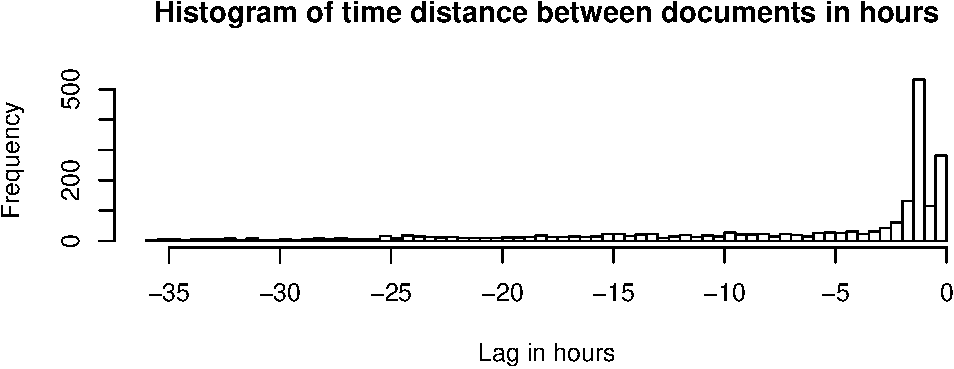
\includegraphics{vignette_files/figure-latex/unnamed-chunk-11-1.pdf}

In the histogram we see that most document pairs with a similarity score
above the threshold are about an hour apart (1 on the x-axis). This is
mainly because the online newspapers often follow the news agency within
a very short amount of time\{\^{}delaynote{]}. As time distance
increases, the number of document pairs decreases, which makes sense
because news gets old fast, so news diffusion should occur within a
limited time after publication.

\subsection{Tailoring the document comparison
window}\label{tailoring-the-document-comparison-window}

If news diffuses from one source to another, then the time difference
cannot be zero, since the source that follows needs time to edit and
publish the news. This delay period can also differ between sources.
Websites can adopt news within minutes, but newspapers have a long time
between pressing and publishing the newspaper, meaning that there is a
period of several hours before publication during which influence is not
possible. Thus, we have to adjust the window for document pairs. To make
it more convenient to adjust and inspect the window settings for
different sources, we offer the \texttt{filter.window} and
\texttt{show.window} functions.

The \texttt{filter.window} function can be used to filter the document
pairs (i.e.~edges) using the \texttt{hour.window} parameter, which works
identical to the \texttt{hour.window} parameter in the
\texttt{documents.window.compare} function. In addition, the
\texttt{from.vertices} and \texttt{to.vertices} parameters can be used
to select the vertices (i.e.~documents) for which this filter is
applied. This makes it easy to tailor the window for different sources,
or source types. For the current data, we use this to set a minimum time
distance of 6 hours for document pairs where the \texttt{to} document is
from a print newspaper.

\begin{Shaded}
\begin{Highlighting}[]
\CommentTok{# set window for all vertices}
\NormalTok{g =}\StringTok{ }\KeywordTok{filter.window}\NormalTok{(g,  }\DataTypeTok{hour.window =} \KeywordTok{c}\NormalTok{(}\FloatTok{0.1}\NormalTok{, }\DecValTok{36}\NormalTok{))}

\CommentTok{# set window for print newspapers}
\NormalTok{g =}\StringTok{ }\KeywordTok{filter.window}\NormalTok{(g,  }\DataTypeTok{hour.window =} \KeywordTok{c}\NormalTok{(}\DecValTok{6}\NormalTok{, }\DecValTok{36}\NormalTok{), }
                  \DataTypeTok{to.vertices =} \KeywordTok{V}\NormalTok{(g)$sourcetype ==}\StringTok{ 'Print NP'}\NormalTok{)}
\end{Highlighting}
\end{Shaded}

For all sources the window has now first been adjusted so that a
document can only match a document that occured at least 0.1 hours
later. For print newspapers, this is then set to 6 hours. With the
\texttt{show.window} function we can view the actual window in the data.
A vertex.attribute can also be given to view the windows grouped by this
attribute.

\begin{Shaded}
\begin{Highlighting}[]
\KeywordTok{show.window}\NormalTok{(g, }\DataTypeTok{vertex.attribute =} \StringTok{'source'}\NormalTok{)}
\end{Highlighting}
\end{Shaded}

\begin{longtable}[c]{@{}lrr@{}}
\toprule
vertex.attribute & window.left & window.right\tabularnewline
\midrule
\endhead
Newsagency & 0.117 & 36.0\tabularnewline
Online NP 1 & 0.117 & 36.0\tabularnewline
Online NP 2 & 0.100 & 34.7\tabularnewline
Print NP 1 & 0.183 & 35.4\tabularnewline
Print NP 2 & 0.800 & 35.4\tabularnewline
\bottomrule
\end{longtable}

\section{Analyzing the document similarity
network}\label{analyzing-the-document-similarity-network}

Before we aggregate the network, it can be informative to look at the
individual sub-components. If a threshold for document similarity is
used, then there should be multiple disconnected components of documents
that are only similar to each other. With the current data, these
components tend to reflect documents that address the same or related
events. Decomposing the network can be done with the
\texttt{decompose.graph()} function from the \texttt{igraph} package.

\begin{Shaded}
\begin{Highlighting}[]
\NormalTok{g_subcomps =}\StringTok{ }\KeywordTok{decompose.graph}\NormalTok{(g)}
\end{Highlighting}
\end{Shaded}

The demo data with the current settings has 685 sub-components. To
visualize these components, we offer the \texttt{plot.document.network}
function. This function draws a network where nodes (i.e.~documents) are
positioned based on their date (x-axis) and source (y-axis).

\begin{Shaded}
\begin{Highlighting}[]
\NormalTok{gs =}\StringTok{ }\NormalTok{g_subcomps[[}\DecValTok{2}\NormalTok{]] }\CommentTok{# select the second sub-component}
\KeywordTok{plot.document.network}\NormalTok{(gs)}
\end{Highlighting}
\end{Shaded}

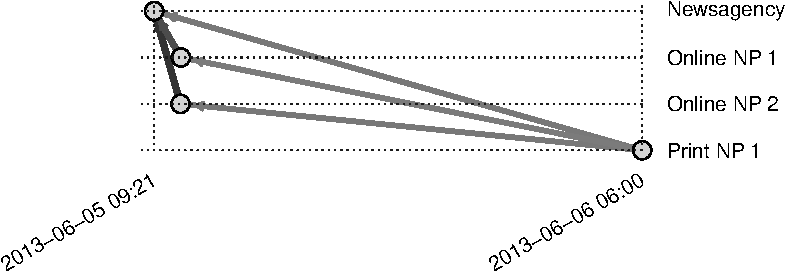
\includegraphics{vignette_files/figure-latex/unnamed-chunk-15-1.pdf}

The visualization shows that a news message was first published by the
news agency on June 5th at 9:21 AM. Soon after this messages was adopted
by two online newspapers, and the next day the print newspaper followed.
The grayscale and width of the edges also show that the online newspaper
messages were more similar (i.e.~thick and black) to the news agency
message compared to the print newspaper message.

By default, the ``source'' attribute is used for the y-axis, but this
can be changed to other document attributes using the
\texttt{source.attribute} parameters. If a DTM is also provided, the
visualization will also include a word cloud with the most frequent
words of these documents.

\begin{Shaded}
\begin{Highlighting}[]
\KeywordTok{plot.document.network}\NormalTok{(gs, }\DataTypeTok{source.attribute =} \StringTok{'sourcetype'}\NormalTok{, }\DataTypeTok{dtm=}\NormalTok{dtm)}
\end{Highlighting}
\end{Shaded}

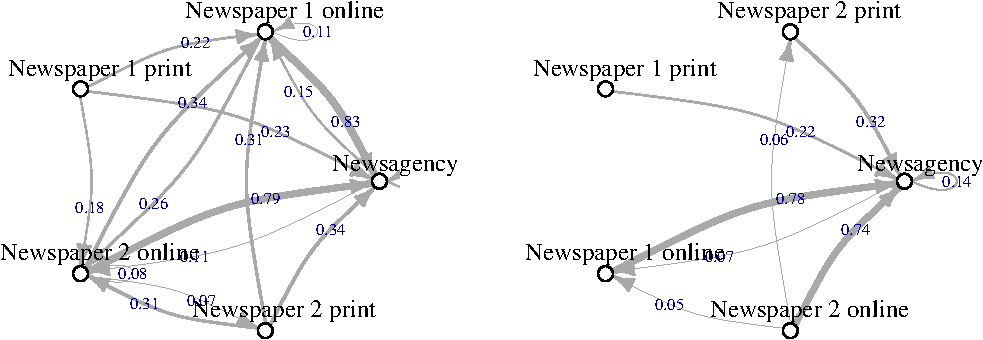
\includegraphics{vignette_files/figure-latex/unnamed-chunk-16-1.pdf}

These visualizations and the corresponding subcomponents help us to
qualitatively investigate specific cases. This also helps to evaluate
whether the document similarity measures are valid given the goal of the
analysis. Furthermore, they illustrate how we can analyze homogeneity
and news diffusion patterns. For each source we can count what
proportion of its publications is similar to earlier publications by
specific other sources. We can also analyze the average time between
publications.

Another usefull application is that we can use them to see whether
certain transformations of the network might be required. Depending on
the purpose of the analysis it can be relevant to add or delete certain
edges. For instance, in the previous visualizations we see that the
print newspaper message matched both the newsagency message and two
online newspaper messages. If we are specifically interested in who the
original source of the message is, then it makes sense to only count the
edge to the newsagency. Here we demonstrate the
\texttt{only.first.match} function, which transforms the network so that
a document only has an edge to the earliest dated document it matches
within the specified time window\footnote{If there are multiple earliest
  dated documents (that is, having the same publication date) then edges
  to all earliest dated documents are kept.}.

\begin{Shaded}
\begin{Highlighting}[]
\NormalTok{gs_onlyfirst =}\StringTok{ }\KeywordTok{only.first.match}\NormalTok{(gs)}
\KeywordTok{plot.document.network}\NormalTok{(gs_onlyfirst)}
\end{Highlighting}
\end{Shaded}

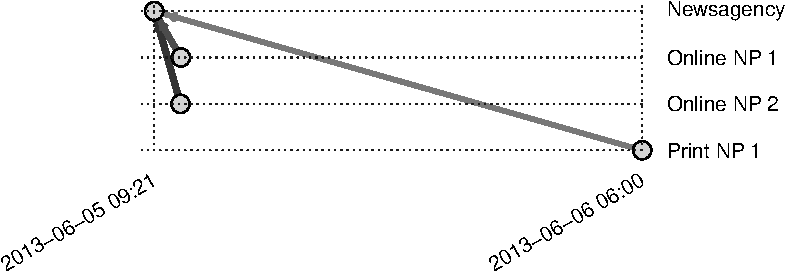
\includegraphics{vignette_files/figure-latex/unnamed-chunk-17-1.pdf}

\subsection{Aggregating the document similarity
network}\label{aggregating-the-document-similarity-network}

This package offers the \texttt{aggregate.network} function as a
versatile way to aggregate the edges of the document similarity network
based on the vertex attributes (i.e.~the document meta information). The
first argument is the network (in the \texttt{igraph} class). The second
argument, for the \texttt{by} parameter, is a character vector to
indicate one or more vertex attributes based on which the edges are
aggregated. Optionally, the \texttt{by} characteristics can also be
specified separately for \texttt{by.from} and \texttt{by.to}. This gives
flexible control over the data, for instance to aggregate \emph{from}
sources \emph{to} sourcetypes, or to aggregate scores for each source
per month.

By default, the function returns the number of edges, as well as the
number of nodes that is connected for both the \texttt{from} and
\texttt{to} group. The number of nodes that is connected is only
relevant if a threshold for similarity (edge weight) is used, so that
whether or not an edge exists indicates whether or not two documents are
similar. In addition, if an \texttt{edge.attribute} is given, this
attribute will be aggregated using the function specified in
\texttt{agg.FUN}. For the following example we include this to analyze
the median of the \texttt{hourdiff} attribute.

\begin{Shaded}
\begin{Highlighting}[]
\NormalTok{g.agg =}\StringTok{ }\KeywordTok{aggregate.network}\NormalTok{(g, }\DataTypeTok{by=}\StringTok{'source'}\NormalTok{, }\DataTypeTok{edge.attribute=}\StringTok{'hourdiff'}\NormalTok{, }\DataTypeTok{agg.FUN=}\NormalTok{median)}

\NormalTok{e =}\StringTok{ }\KeywordTok{get.data.frame}\NormalTok{(g.agg, }\StringTok{'edges'}\NormalTok{)}
\KeywordTok{head}\NormalTok{(e)}
\end{Highlighting}
\end{Shaded}

\begin{longtable}[c]{@{}llrrrrrr@{}}
\toprule
from & to & edges & agg.hourdiff & from.V & from.Vprop & to.V &
to.Vprop\tabularnewline
\midrule
\endhead
Newsagency & Newsagency & 114 & 8.49 & 94 & 0.157 & 98 &
0.164\tabularnewline
Print NP 1 & Newsagency & 19 & 8.33 & 15 & 0.102 & 18 &
0.030\tabularnewline
Online NP 1 & Newsagency & 103 & 4.88 & 81 & 0.175 & 92 &
0.154\tabularnewline
Online NP 2 & Newsagency & 67 & 6.78 & 58 & 0.139 & 61 &
0.102\tabularnewline
Print NP 2 & Newsagency & 10 & 10.75 & 10 & 0.076 & 10 &
0.017\tabularnewline
Newsagency & Online NP 1 & 434 & 1.27 & 380 & 0.637 & 406 &
0.879\tabularnewline
\bottomrule
\end{longtable}

In the edges of the aggregated network there are six scores for each
edge. The \texttt{edges} attribute counts the number of edges from the
\texttt{from} group to the \texttt{to} group. For example, we see that
\emph{Newsagency} documents have 434 edges to later published
\emph{Online NP 1} documents. The \texttt{agg.hourdiff} attribute shows
that the median of the hourdiff attribute of these 434 edges is 1.27 (1
hour and 16 minutes). In addition to the edges, we can look at the
number of messages (i.e.~vertices) in the \texttt{from} group that
matched with at least one message in the \texttt{to} group. This is
given by the \texttt{from.V} attribute, which shows here that 380
\emph{Newsagency} documents matched with a later published \emph{Online
NP 1} document\footnote{Note that the \texttt{edges} score is always
  equal to or higher than the \texttt{from.matched} score, since one
  document can match with multiple other documents.}. This is also given
as the proportion of all vertices/documents in the \texttt{from} group,
as the \texttt{from.Vprop} attribute. Substantially, the
\texttt{from.Vprop} score thus indicates that 63.65\% of political news
messages in \emph{Newsagency} is similar or identical to later published
\emph{Online NP 1} messages.

Alternatively, we can also look at the \emph{to.V} and \emph{to.Vprop}
scores to focus on the number and proportion of messages in the
\texttt{to} group that match with at least one message in the
\texttt{from} group. Here we see, for instance, that 87.88\% of
political news messages in \emph{Online NP 1} is similar to or identical
to previously published messages \emph{Newsagency} messages. The
\emph{from.Vprop} and \emph{to.Vprop} scores thus give different and
complementary measures for the influence of \emph{Newsagency} on
\emph{Online NP 1}.

\subsection{Inspecting and visualizing
results}\label{inspecting-and-visualizing-results}

The final step is to interpret the aggregated network data, or to
prepare this data for use in a different analysis. We already saw that
the network data can be transformed to a common data.frame with the
\texttt{get.data.frame} function. Alternatively, \texttt{igraph} has the
\texttt{get.adjacency} function to return the values for one edge
attribute as an adjacency matrix, with the vertices in the rows and
columns. This is a good way to present the scores of the aggregated
network.

\begin{Shaded}
\begin{Highlighting}[]
\NormalTok{adj.m =}\StringTok{ }\KeywordTok{get.adjacency}\NormalTok{(g.agg, }\DataTypeTok{attr=} \StringTok{'to.Vprop'}\NormalTok{, }\DataTypeTok{sparse =} \NormalTok{F)}
\KeywordTok{round}\NormalTok{(adj.m, }\DecValTok{2}\NormalTok{) }\CommentTok{# round on 2 decimals}
\end{Highlighting}
\end{Shaded}

\begin{longtable}[c]{@{}lrrrrr@{}}
\toprule
& Newsagency & Print NP 1 & Online NP 1 & Online NP 2 & Print NP
2\tabularnewline
\midrule
\endhead
Newsagency & 0.16 & 0.24 & 0.88 & 0.82 & 0.34\tabularnewline
Print NP 1 & 0.03 & 0.03 & 0.05 & 0.04 & 0.02\tabularnewline
Online NP 1 & 0.15 & 0.22 & 0.11 & 0.33 & 0.31\tabularnewline
Online NP 2 & 0.10 & 0.18 & 0.26 & 0.08 & 0.31\tabularnewline
Print NP 2 & 0.02 & 0.01 & 0.03 & 0.07 & 0.01\tabularnewline
\bottomrule
\end{longtable}

Alternatively, an intuitive way to present the aggregated network is by
visualizing it. For this we can use the visualization features of the
\texttt{igraph} package. To make this more convenient, we also offer the
\texttt{plot.aggregate.network} function. This is a wrapper for the
plot.igraph function, which makes it easier to use different edge weight
attributes and to use an edge threshold, and has default plotting
parameters to work well for directed graphs with edge labels. For this
example we use the \texttt{to.Vprop} edge attribute with a threshold of
0.2.

\begin{Shaded}
\begin{Highlighting}[]
\KeywordTok{plot.aggregate.network}\NormalTok{(g.agg, }\DataTypeTok{weight.var =} \StringTok{'to.Vprop'}\NormalTok{,}
                       \DataTypeTok{weight.thres =} \FloatTok{0.2}\NormalTok{)}
\end{Highlighting}
\end{Shaded}

\begin{center}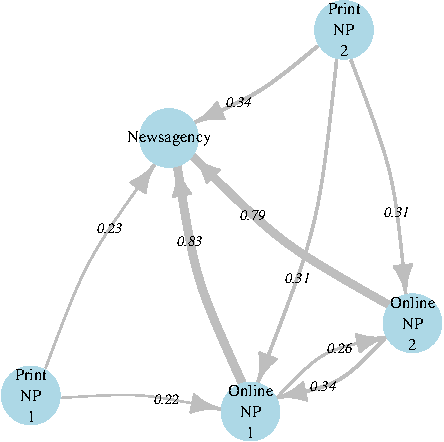
\includegraphics{vignette_files/figure-latex/unnamed-chunk-20-1} \end{center}

For illustration, we can now see how the results change if we transform
the network with the \texttt{only.first.match} function, which only
counts edges to the first source that published a document.

\begin{Shaded}
\begin{Highlighting}[]
\NormalTok{g2 =}\StringTok{ }\KeywordTok{only.first.match}\NormalTok{(g)}
\NormalTok{g2.agg =}\StringTok{ }\KeywordTok{aggregate.network}\NormalTok{(g2, }\DataTypeTok{by=}\StringTok{'source'}\NormalTok{, }\DataTypeTok{edge.attribute=}\StringTok{'hourdiff'}\NormalTok{, }\DataTypeTok{agg.FUN=}\NormalTok{median)}

\KeywordTok{plot.aggregate.network}\NormalTok{(g2.agg, }\DataTypeTok{weight.var =} \StringTok{'to.Vprop'}\NormalTok{,}
                       \DataTypeTok{weight.thres =} \FloatTok{0.2}\NormalTok{)}
\end{Highlighting}
\end{Shaded}

\begin{center}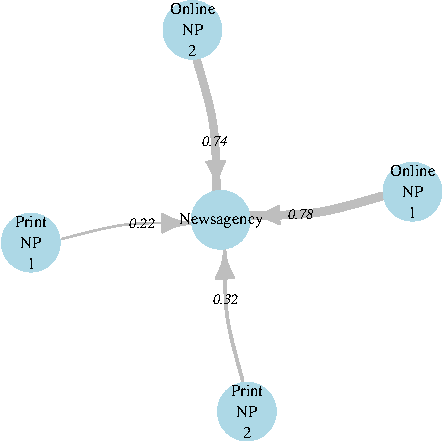
\includegraphics{vignette_files/figure-latex/unnamed-chunk-21-1} \end{center}

The first network is much more dense compared to the second. In
particular, we see stronger edges between the print and online editions
of the newspapers. In the second network almost only the ties to the
news agency remain. This implies that many of the edges between
newspapers in the first network resulted from cases where both
newspapers adopt the same news agency articles.

Note that the second network is not better per se. It is possible that
the initial source of a message is not the direct source. For example, a
blog might not have acces to the news agency feed, and therefore only
receive news agency messages if they are published by another source.
Thus, the most suitable approach depends on the purpose of the analysis.
One of the goals of creating this package is to facilitate a platform
for scholars and professionals to develop best practises for different
occasions.

\subsection{Alternative applications of this
package}\label{alternative-applications-of-this-package}

There are several alternative applications of the functions offered in
this package that are not covered in this vignette. Here we briefly
point out some of the more usefull alternatives.

In the aggregate.network function it is possible to use different vertex
attributes to aggregate the edges for \texttt{from} and \texttt{to}
nodes. A particularlly interesting application of this feature is to use
the publication date in the aggregation. For instance, with the
following settings, we can get the proportion of matched documents per
day. Here we also demonstrate the \texttt{return.df} parameter in the
\texttt{aggregate.network} function. This way the results are returned
as a single data.frame in which relevant edge and vertex information is
merged.

\begin{Shaded}
\begin{Highlighting}[]
\KeywordTok{V}\NormalTok{(g)$day =}\StringTok{ }\KeywordTok{format}\NormalTok{(}\KeywordTok{as.Date}\NormalTok{(}\KeywordTok{V}\NormalTok{(g)$date), }\StringTok{'%Y-%m-%d'}\NormalTok{)}
\NormalTok{agg.perday =}\StringTok{ }\KeywordTok{aggregate.network}\NormalTok{(g, }\DataTypeTok{by.from=}\StringTok{'sourcetype'}\NormalTok{, }\DataTypeTok{by.to=}\KeywordTok{c}\NormalTok{(}\StringTok{'sourcetype'}\NormalTok{, }\StringTok{'day'}\NormalTok{), }
                                  \DataTypeTok{edge.attribute=}\StringTok{'hourdiff'}\NormalTok{, }\DataTypeTok{agg.FUN=}\NormalTok{median, }
                                  \DataTypeTok{return.df=}\NormalTok{T)}


\KeywordTok{head}\NormalTok{(agg.perday[agg.perday$to.sourcetype ==}\StringTok{ 'Online NP'}\NormalTok{,  }
                \KeywordTok{c}\NormalTok{(}\StringTok{'from.sourcetype'}\NormalTok{, }\StringTok{'to.sourcetype'}\NormalTok{, }\StringTok{'to.day'}\NormalTok{,}\StringTok{'to.Vprop'}\NormalTok{)])}
\end{Highlighting}
\end{Shaded}

\begin{longtable}[c]{@{}llllr@{}}
\toprule
& from.sourcetype & to.sourcetype & to.day & to.Vprop\tabularnewline
\midrule
\endhead
64 & Print NP & Online NP & 2013-06-01 & 0.263\tabularnewline
65 & Newsagency & Online NP & 2013-06-01 & 0.789\tabularnewline
66 & Online NP & Online NP & 2013-06-01 & 0.368\tabularnewline
67 & Newsagency & Online NP & 2013-06-02 & 0.778\tabularnewline
68 & Online NP & Online NP & 2013-06-02 & 0.111\tabularnewline
69 & Newsagency & Online NP & 2013-06-03 & 0.864\tabularnewline
\bottomrule
\end{longtable}

Looking at the \emph{to.Vprop} score, we see that on 2013-06-01, 78.95\%
of \emph{Online NP} messages match with previously published
\emph{Newsagency} message\footnote{Note that that \emph{from.Vprop}
  cannot be interpreted in the same way, because it gives the proportion
  of all messages in the \texttt{from} group. If one is interested in
  the \emph{from.Vprop} score per day, the \emph{by.from} and
  \emph{by.to} arguments in \emph{aggregate.network} can be switched.}.
This way, the aggregated document similarity data can be analyzed as a
time-series. For instance, to analyze whether certain developments
affect content homogeneity or intermedia dynamics. Also, it enables us
to analyze the mean of the aggregated results over time. The
\texttt{return.df} feature is convenient for this purpose, because it
directly matches all the vertex and edge attributes (as opposed to the
\texttt{get.data.frame} function).

Another usefull application of this feature is to only aggregate the
\texttt{by.to} group, by using the document name in the \texttt{by.from}
argument. This way, the data in the \emph{by.to} group is aggregated for
each individual message. In the following example we use this to see for
each individual message whether it matches with later published messages
in each sourcetype. This could for instance be used to analyze whether
certain document level variables (e.g., news factors, sensationalism)
make a message more likely to be adopted by other news outlets. We set
the \texttt{edge.attribute} to ``weight'' and \texttt{agg.FUN} to max,
so that for each document we can see how strong the strongest match with
each source was.

\begin{Shaded}
\begin{Highlighting}[]
\NormalTok{agg.perdoc =}\StringTok{ }\KeywordTok{aggregate.network}\NormalTok{(g, }\DataTypeTok{by.from=}\StringTok{'name'}\NormalTok{, }\DataTypeTok{by.to=}\StringTok{'sourcetype'}\NormalTok{, }
                                  \DataTypeTok{edge.attribute=}\StringTok{'weight'}\NormalTok{, }\DataTypeTok{agg.FUN=}\NormalTok{max, }
                                  \DataTypeTok{return.df=}\NormalTok{T)}
\NormalTok{docXsource =}\StringTok{ }\KeywordTok{xtabs}\NormalTok{(agg.weight ~}\StringTok{ }\NormalTok{from.name +}\StringTok{ }\NormalTok{to.sourcetype, agg.perdoc, }\DataTypeTok{sparse =} \NormalTok{F)}
\KeywordTok{head}\NormalTok{(docXsource)}
\end{Highlighting}
\end{Shaded}

\begin{longtable}[c]{@{}lrrr@{}}
\toprule
& Newsagency & Online NP & Print NP\tabularnewline
\midrule
\endhead
147908507 & 0.40 & 0.425 & 0\tabularnewline
148662598 & 0.00 & 0.767 & 0\tabularnewline
150454094 & 0.52 & 0.528 & 0\tabularnewline
150454102 & 0.00 & 0.895 & 0\tabularnewline
150454110 & 0.00 & 0.402 & 0\tabularnewline
150454167 & 0.00 & 0.996 & 0\tabularnewline
\bottomrule
\end{longtable}

Finally, note that we have now only compared documents with future
documents. We thereby focus the analysis on news diffusion. To focus on
content homogeneity, each document can be compared to both past and
future documents. By measuring content homogeneity aggregated over time,
patterns such as longitudinal trends can be analyzed.

\section{Conclusion and future
improvements}\label{conclusion-and-future-improvements}

We have demonstrated how the \emph{newsflow} package can be used to
perform a many-to-many comparison of documents. The primary focus and
most important feature of this package is the
\texttt{documents.window.compare} function. This function compares all
documents that occur within a given time distance, which makes it
computationally feasible for longitudinal data. Using this data, we can
analyze to what extent different sources publish the same content and
whether there are consistent patterns in who follows whom. The secondary
focus of this package is to provide functions to organize, visualize and
analyze the document similarity data within R. By enabling both the
document comparison and analysis to be performed within R, this type of
analysis becomes more accesible to scholars less versed in computational
text analysis, and it becomes easier to share and replicate this type of
research.

The data input required for this analysis consists solely of textual
documents and their corresponding publication date and source. Since no
human coding is required, the package enables large scale comparative
and longitudinal studies. Although the demonstration in this vignette
used a moderate sized dataset, the \texttt{document.window.compare} can
handle much larger data and is fast, thanks to the excellent sparse
matrix multiplication alghoritm of the \texttt{Matrix} package.

The validity of the method presented here relies on various factors;
most importantly the type of data, the pre-processing and DTM
preparation steps and the similarity threshold. It is thus recommended
to use a gold standard, based on human interpretation, to test its
validity. In a recent empirical study (author citation, forthcoming) we
obtained good performance for whether documents addressed the same
events and whether they contained identical phrases by determining
thresholds based on a manually coded gold standard. Also, by using a
news website that consistently referred to a news agency by name, we
confirmed that we could reliably identify news agency influence for this
format. Naturally, there are always limitations to the accuracy with
which influence in news diffusion can be measured using only content
analysis. However, we generally do not have access to other reliable
information. The advantage of a content analysis based approach is that
it can be used on a large scale and over long periods of time, without
relying on often equally inaccurate self-reports of news workers. The
current package contributes to the toolkit for this type of analysis.

Our goal is to continue developing this package as a specialized toolkit
for analyzing the homogeneity and diffusion of news content. First of
all, additional approaches for measuring whether documents are related
will be added. Currently only a vector space model approach for
calculating document similarity is implemented. For future versions
alternative approaches such as language modeling will also be explored.
In particular, we want to add measures to express the relation of
documents over time in terms of probability and information gain. This
would also allow us to define a more formal criterion for whether or not
a relation exists, other than using a constant threshold for document
similarity. Secondly, new methods for analyzing and visualizing the
network data will be explored. In particular, methods will be
implemented for analyzing patterns beyond dyadic ties between news
outlets, building on techniques from the field of network analysis. To
promote the involvement of other scholars and professionals in this
development, the package is published entirely open-source. The source
code is hosted on
GitHub--\emph{\url{https://github.com/kasperwelbers/newsflow}}.

\section{Practical code example}\label{practical-code-example}

\begin{Shaded}
\begin{Highlighting}[]
\KeywordTok{library}\NormalTok{(newsflow)}

\CommentTok{# Prepare DTM and meta data}
\KeywordTok{data}\NormalTok{(dtm)}
\KeywordTok{data}\NormalTok{(meta)}

\NormalTok{tdd =}\StringTok{ }\KeywordTok{term.day.dist}\NormalTok{(dtm, meta)}
\NormalTok{dtm =}\StringTok{ }\NormalTok{dtm[,tdd$term[tdd$days.entropy.norm <=}\StringTok{ }\FloatTok{0.3}\NormalTok{]]}

\NormalTok{dtm =}\StringTok{ }\KeywordTok{weightTfIdf}\NormalTok{(dtm)}

\CommentTok{# Prepare document similarity network}
\NormalTok{g =}\StringTok{ }\KeywordTok{documents.window.compare}\NormalTok{(dtm, meta, }\DataTypeTok{hour.window =} \KeywordTok{c}\NormalTok{(}\FloatTok{0.1}\NormalTok{,}\DecValTok{36}\NormalTok{), }\DataTypeTok{min.similarity =} \FloatTok{0.4}\NormalTok{)}
\NormalTok{g =}\StringTok{ }\KeywordTok{filter.window}\NormalTok{(g, }\DataTypeTok{hour.window =} \KeywordTok{c}\NormalTok{(}\DecValTok{6}\NormalTok{, }\DecValTok{36}\NormalTok{), }\KeywordTok{V}\NormalTok{(g)$sourcetype ==}\StringTok{ 'Print NP'}\NormalTok{)}

\NormalTok{g_subcomps =}\StringTok{ }\KeywordTok{decompose.graph}\NormalTok{(g)}
\KeywordTok{plot.document.network}\NormalTok{(g_subcomps[[}\DecValTok{2}\NormalTok{]], }\DataTypeTok{dtm=}\NormalTok{dtm)}

\CommentTok{# Aggregate network }
\NormalTok{g.agg =}\StringTok{ }\KeywordTok{aggregate.network}\NormalTok{(g, }\DataTypeTok{by=}\StringTok{'source'}\NormalTok{, }\DataTypeTok{edge.attribute=}\StringTok{'hourdiff'}\NormalTok{, }\DataTypeTok{agg.FUN=}\NormalTok{median)}

\KeywordTok{get.adjacency}\NormalTok{(g.agg, }\DataTypeTok{attr=}\StringTok{'to.Vprop'}\NormalTok{)}
\KeywordTok{plot.aggregate.network}\NormalTok{(g.agg, }\DataTypeTok{weight.var =} \StringTok{'to.Vprop'}\NormalTok{, }\DataTypeTok{weight.thres=}\FloatTok{0.2}\NormalTok{)}

\NormalTok{g2 =}\StringTok{ }\KeywordTok{only.first.match}\NormalTok{(g)}
\NormalTok{g2.agg =}\StringTok{ }\KeywordTok{aggregate.network}\NormalTok{(g2, }\DataTypeTok{by=}\StringTok{'source'}\NormalTok{, }\DataTypeTok{edge.attribute=}\StringTok{'hourdiff'}\NormalTok{, }\DataTypeTok{agg.FUN=}\NormalTok{median)}

\KeywordTok{get.adjacency}\NormalTok{(g2.agg, }\DataTypeTok{attr=}\StringTok{'to.Vprop'}\NormalTok{)}
\KeywordTok{plot.aggregate.network}\NormalTok{(g2.agg, }\DataTypeTok{weight.var =} \StringTok{'to.Vprop'}\NormalTok{, }\DataTypeTok{weight.thres=}\FloatTok{0.2}\NormalTok{)}
\end{Highlighting}
\end{Shaded}

\renewcommand\refname{References}
\bibliography{references}

\end{document}
